\documentclass[../../main.tex]{subfiles}

\begin{document}

\setchapterpreamble[u]{\margintoc}

\chapter{排序的应用}

在链表中,我们已经实现了某些基础排序的应用,在本章我们通过简单介绍一下排序的应用。实际上排序更多的是
一种思想,我们更应该掌握使用排序的思想解决问题。

\section{基于比较的排序算法}

本节首先基于\href{https://leetcode.cn/problems/sort-an-array/}{排序数组}阐述所有的基于比较的排序算法。

\subsection{插入排序}

插入排序的做法相当简单,我们只需要理解其循环不变量就可以解决该问题,其循环不变量为:\texttt{[0, i)}
是有序的,我们每次将\texttt{nums[i]}插入到\texttt{[0, i)}中,然后\texttt{i++},直到\texttt{i}等于
\texttt{nums.length}。

\lstinputlisting[language=C++]{code/sort-an-array-insertion-sort.cpp}

\subsection{选择排序}

选择排序的做法也相当简单,我们同样需要理解其循环不变量,其循环不变量为:\texttt{[0, i)}是有序的,
我们每次选择\texttt{[i, nums.length)}中的最小值,然后将其与\texttt{nums[i]}交换,然后\texttt{i++},
直到\texttt{i}等于\texttt{nums.length}。

\lstinputlisting[language=C++]{code/sort-an-array-selection-sort.cpp}

\subsection{冒泡排序}

冒泡排序的做法也相当简单。我们同样需要理解其循环不变量,其循环不变量为:\texttt{[0, i)}是有序的,然后
倒序地遍历\texttt{[i + 1, nums.length)},将最小值不断交换到\texttt{nums[i]},然后\texttt{i++},
直到\texttt{i}等于\texttt{nums.length}。

\lstinputlisting[language=C++]{code/sort-an-array-buddle-sort.cpp}

\subsection{归并排序}

我们已经在链表章节中的\ref{subsec:sort-list}实现了归并排序,这里我们再次实现一下,其实现与链表中的实现相同,
只是链表的操作是离散的,而数组的操作是连续的,因此我们需要构建新的数组来存储归并的结果。

显然关键的操作仍然是合并两个有序数组。其操作很简单,最关键的问题在于如果我们遇到了某个数组的末尾,我们应该怎么处理。
简单的想法就是写很多个判断语句,但是这样的代码很难维护,我们可以使用哨兵来解决这个问题,我们可以在两个数组的末尾
分别添加一个最大值,这样我们就不需要判断数组是否到达了末尾,而只需要比较两个数组的当前元素的大小即可\sidenote{
  这是一个很常见的思路方式。
}。

\lstinputlisting[language=C++]{code/sort-an-array-divide-and-conquer.cpp}

\subsection{快速排序}

快速排序的核心仍然是对数组进行分割,我们可以选择数组的末尾元素作为\texttt{pivot},然后将数组分割为两部分,
一部分是小于\texttt{pivot}的,另一部分是大于\texttt{pivot}的,然后递归地对这两部分进行处理。实际上我们
在链表中的\ref{subsec:partition-list}已经完成了对链表的分割,由于链表是离散的,分割是比较简单的。

我使用两个指针一个\texttt{i}指向小于\texttt{pivot}的最后一个元素,另一个\texttt{j}指向当前元素,
也就是\texttt{[0, i]}都是小于\texttt{pivot}的,\texttt{[i + 1, j - 1]}是大于\texttt{pivot}的,
\texttt{[j, nums.length)}是未处理的元素。这样我们每次只需要判断\texttt{nums[j]}是否
小于\texttt{pivot},如果小于,我们就将\texttt{nums[j]}与\texttt{nums[i + 1]}交换,然后
\texttt{i++},\texttt{j++},否则只需要\texttt{j++}即可\sidenote{实际上,这个方法是算法导论
中采用的方法,我认为是非常设计的好的算法,其循环不变量十分优雅。}。

\lstinputlisting[language=C++]{code/sort-an-array-quick-sort.cpp}

\subsection{堆排序}

使用堆排序是可谓最为复杂的一个排序了(前提当然是你不使用标准库提供的优先队列)。主要是需要去定义
堆的数据结构即可,这是一个基础知识\sidenote{在此处,我并没有具体阐述堆这个数据结构,如果你
不了解这个数据结构,我推荐你阅读算法导论的第6章,对堆排序这个问题进行了非常严格的数学证明。}。

\lstinputlisting[language=C++]{code/sort-an-array-heap-sort.cpp}

\section{基于计数的排序算法}

\subsection{\href{https://leetcode.cn/problems/sort-colors/}{颜色分类}}

这个题是计数排序的简单应用,我们可以使用计数排序的思想,先统计每个颜色的个数,然后再将其填充到数组中即可。
因为者有三个数字,所以我们可以只用常数空间解决这个问题。

\lstinputlisting[language=C++]{code/sort-colors.cpp}

\section{排序的应用}

\subsection{\href{https://leetcode.cn/problems/kth-largest-element-in-an-array/}
{数组中的第K个最大元素}}

我们应该如何选择数组中的第K个最大元素呢?我们可以先对数组进行排序,然后选择第K个元素,但是这样的
时间复杂度为$O(n\log n)$,我们可以使用快速排序的思想,每次选择一个元素,将数组分为两部分,然后
判断第K个元素在哪一部分,然后递归的进行查找。这样时间的复杂度为$O(n)$\sidenote{要证明这个时间
的复杂度为$O(n)$,需要通过概率来证明,证明方法可以参考算法导论。}。

我们仍然以例子说明,我们取末尾的元素作为\texttt{pivot},然后按照这个数字,对数组进行分割,然后
递归地进行处理。假设我们对最初的数组完成了以下的分割,并得到了这个\texttt{pivot}的位置,如下图
所示:

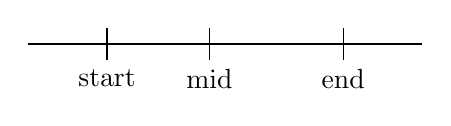
\begin{tikzpicture}
  \draw (0,0) -- (5,0);
  \draw (2.3,-0.2) node[below] {mid} -- (2.3,0.2);
  \draw (1,0.2) -- (1,-0.2) node[below] {start};
  \draw (4,0.2) -- (4,-0.2) node[below] {end};
\end{tikzpicture}

如上图所示,我们首先计算出当前的\texttt{mid}距离\texttt{start}的距离,其值为
\texttt{mid - start + 1},然后我们对这个值进行相应的判断:

\begin{itemize}
  \item 如果其等于\texttt{k},那么证明我们找到了第\texttt{k}个最大元素。
  \item 如果其大于\texttt{k},那么我们递归的对左边的数组进行处理,首先我们要确定新的
  \texttt{start}和\texttt{end},\texttt{start}不变,\texttt{end}变为\texttt{mid - 1}。
  同时\texttt{k}不变。
  \item 如果其小于\texttt{k},那么我们递归的对右边的数组进行处理,首先我们要确定新的
  \texttt{start}和\texttt{end},\texttt{start}变为\texttt{mid + 1},\texttt{end}不变。
  同时\texttt{k}变为\texttt{k - (mid - start + 1)}。
\end{itemize}

然后,我们就可以给出如下的代码:

\lstinputlisting[language=C++]{code/kth-largest-element-in-an-array.cpp}

\end{document}
